\chapter{User Manual}

This section explains how to download and install the software.

\section{Outlier Orchestrator}

\subsection{Requirements}

To run the outlier orchestrator, there are some software requirements that must be satisfied.

\begin{itemize}
    \item \texttt{Node.js:} v $\geq$ v22.17.1
    \item \texttt{\ac{npm}:} v $\geq$ 10.9.2
\end{itemize}

\subsection{Installation}

Clone the repository available in \autocite{OutlierClassifierOutlier_orchestrator2025a}. Install the dependencies with 

\begin{lstlisting}[caption={Using \ac{npm} to install dependencies}]
    npm install 
\end{lstlisting}

Run the outlier orchestrator with

\begin{lstlisting}[caption={Running the outlier orchestrator}]
    npm start
\end{lstlisting}

Access \hyperbaseurl{http://localhost:3000/}{\texttt{http://localhost:3000/}} on any browser. The outlier frontend must be shown. Backend is already running.

\section{Outlier models}

To run any python model, some requirements must be satisfied:

\begin{itemize}
    \item \textbf{Python version $\geq$ 3.11}
    \item \textbf{FastAPI}
    \item \textbf{scikit-learn}
\end{itemize}

Then clone the repositories containing any model. Execute the \texttt{main.py} file, and copy the displayed port.

On the outlier frontend, select the "add model" button, which is located in the top-right corner. Then, four dialogs will be displayed, where the first one asks for the model name, and the following for the model's endpoints for training, predicting, and health status.

If the provided data is correct, model will start receiving health messages, and the frontend will set the model as online.\ \autoref{fig:model-boot} demonstrates this behavior, where on the left the orchestrator frontend is shown, on the top-right window the orchestrator backend logs show that XGBoost is offline, and \ac{IForest} is receiving health check messages.

\begin{figure}[H]
    \centering
    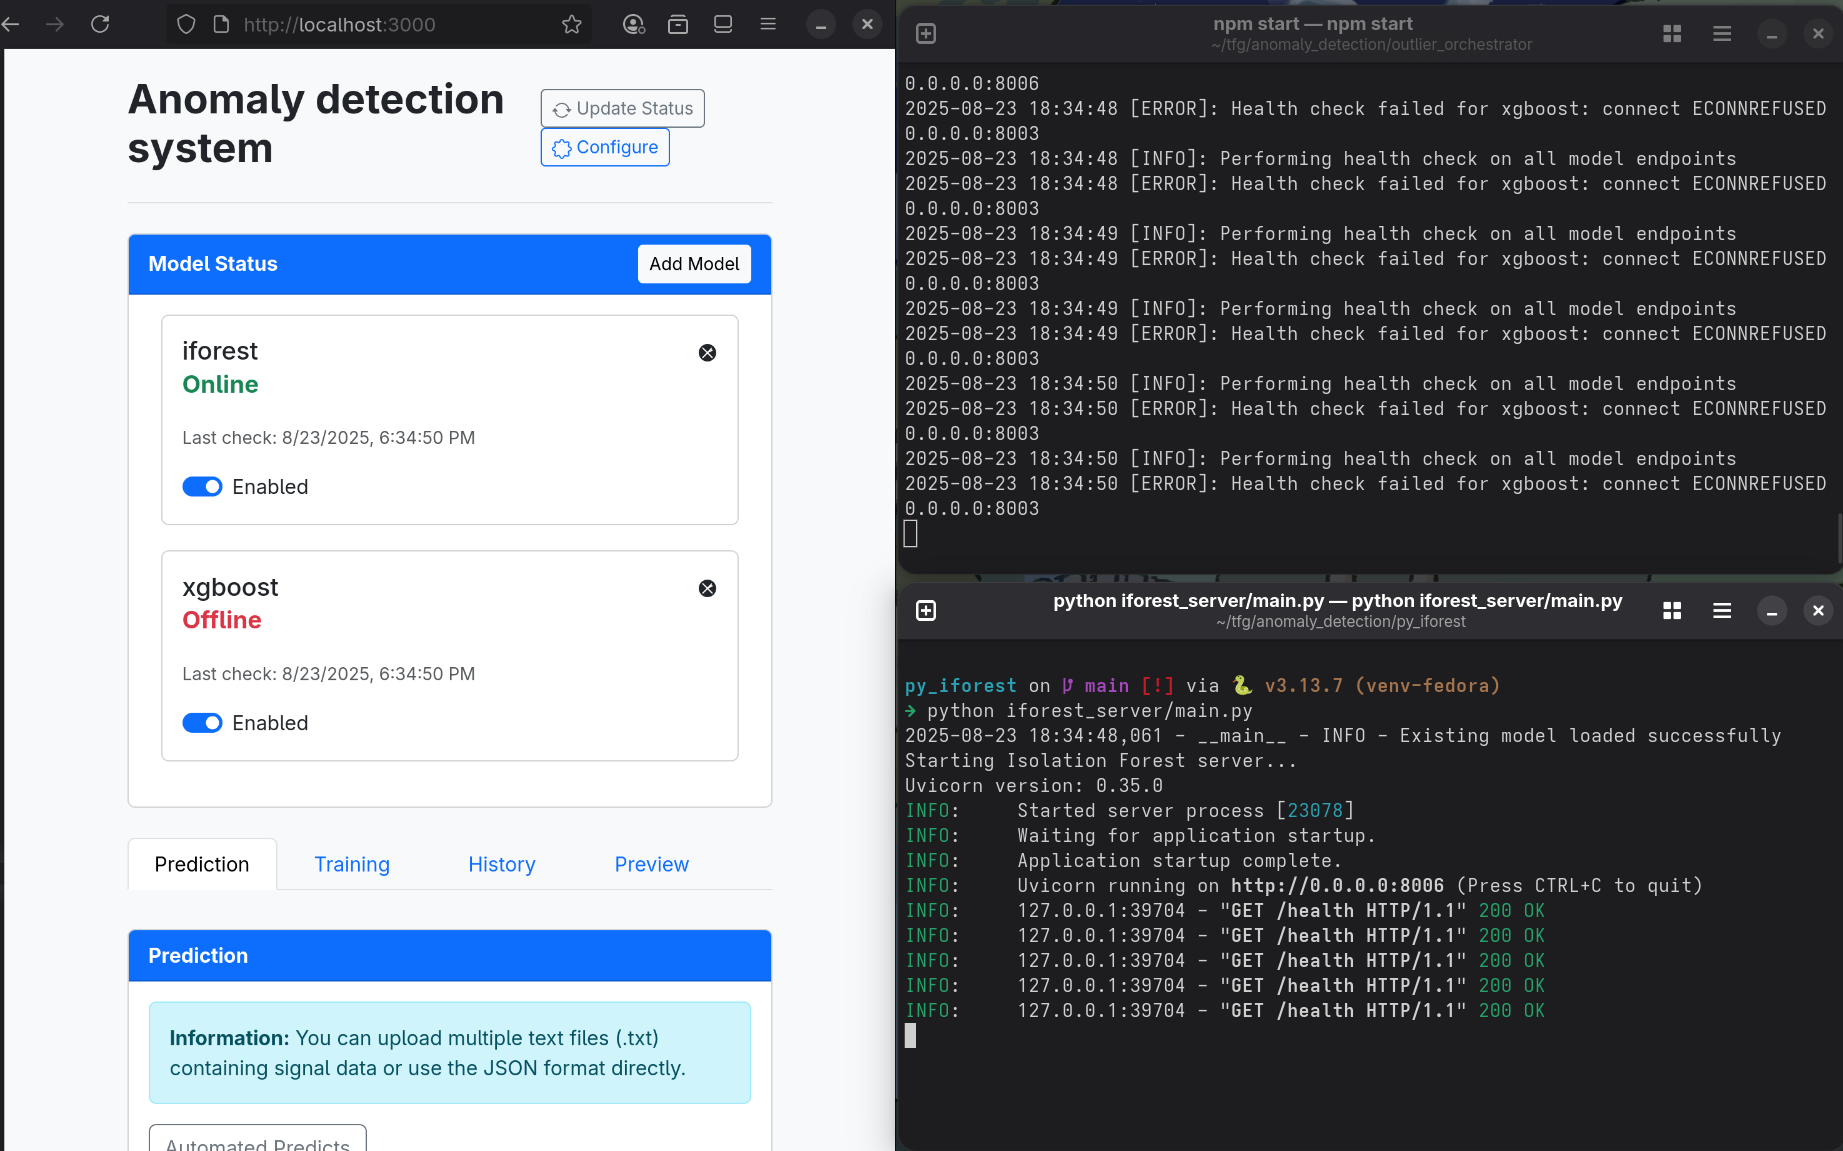
\includegraphics[width=\textwidth]{apendix/model-online.png}
    \caption{Demonstration of booting a model}
    \label{fig:model-boot}
\end{figure}
